\documentclass[12pt]{article}
\usepackage{enumitem}
\usepackage{amsmath}
\usepackage{graphicx}
\usepackage{listings}

\title{EECS 151/251A - LB\\ RISC-V FPGA Project}
\author{Alejandro Sierra \\ Jakob Peter Karg\\ UC Berkeley}
\date{Spring 2017}


\begin{document}
\maketitle

\section{Design objectives}

The goal of this project was to implement a complete version of a RISC-V CPU with a three stage pipeline. The CPU was implemented using Verilog and targeted the VIRTEX 5 LX110T FPGA by Xilinx.

\subsection{Pipeline}
\label{sub:pipeline-intro}
The CPU was implemented with a three stage pipeline. Because the memory is implemented using synchronous bram blocks, two of the three stages were fixed to be at the instruction- and data-memory. We decided to put the third stage in between the register file and the ALU.

\subsection{Memory hierarchy}

The instruction- and data-memory are implemented using synchronous bram blocks. There are three memories: The instruction memory, the data memory and the BIOS memory. The BIOS memory is a read-only memory which contains the BIOS, which is executed when the CPU gets reset. The BIOS can read instructions over the UART and write them to the instruction memory. This way, the processor can be programmed to execute a program over UART.
We are using memory-mapped IO to connect to various peripherals. We implemented a memory-read- and a memory-write-controller that map the addresses to the corresponding memory / IO device.

\section{High-Level organization}
The CPU is broken up into three pipeline stages as described in \ref{sub:pipeline-intro}. The first stage contains the instruction memory, the register file and the control logic for the next pc. The second stage contains the ALU as well as the calculation of the branch address and the branch condition and a memory write controller. The third stage contains the data memory and the memory mapped IO, the memory read controller and the writeback to the register file. In parallel to all of that there is the control unit, which takes in the instruction in the first stage and calculates the control signals for all multiplexers in the CPU. It detects data hazards and forwards the data through the necessary multiplexers. It also detects control flow hazards and sets the multiplexer which controls the next pc and kills the instruction in the second stage if necessary.
The block diagram can be seen in figure \ref{fig:block-diagram}.

\begin{figure}[!p]
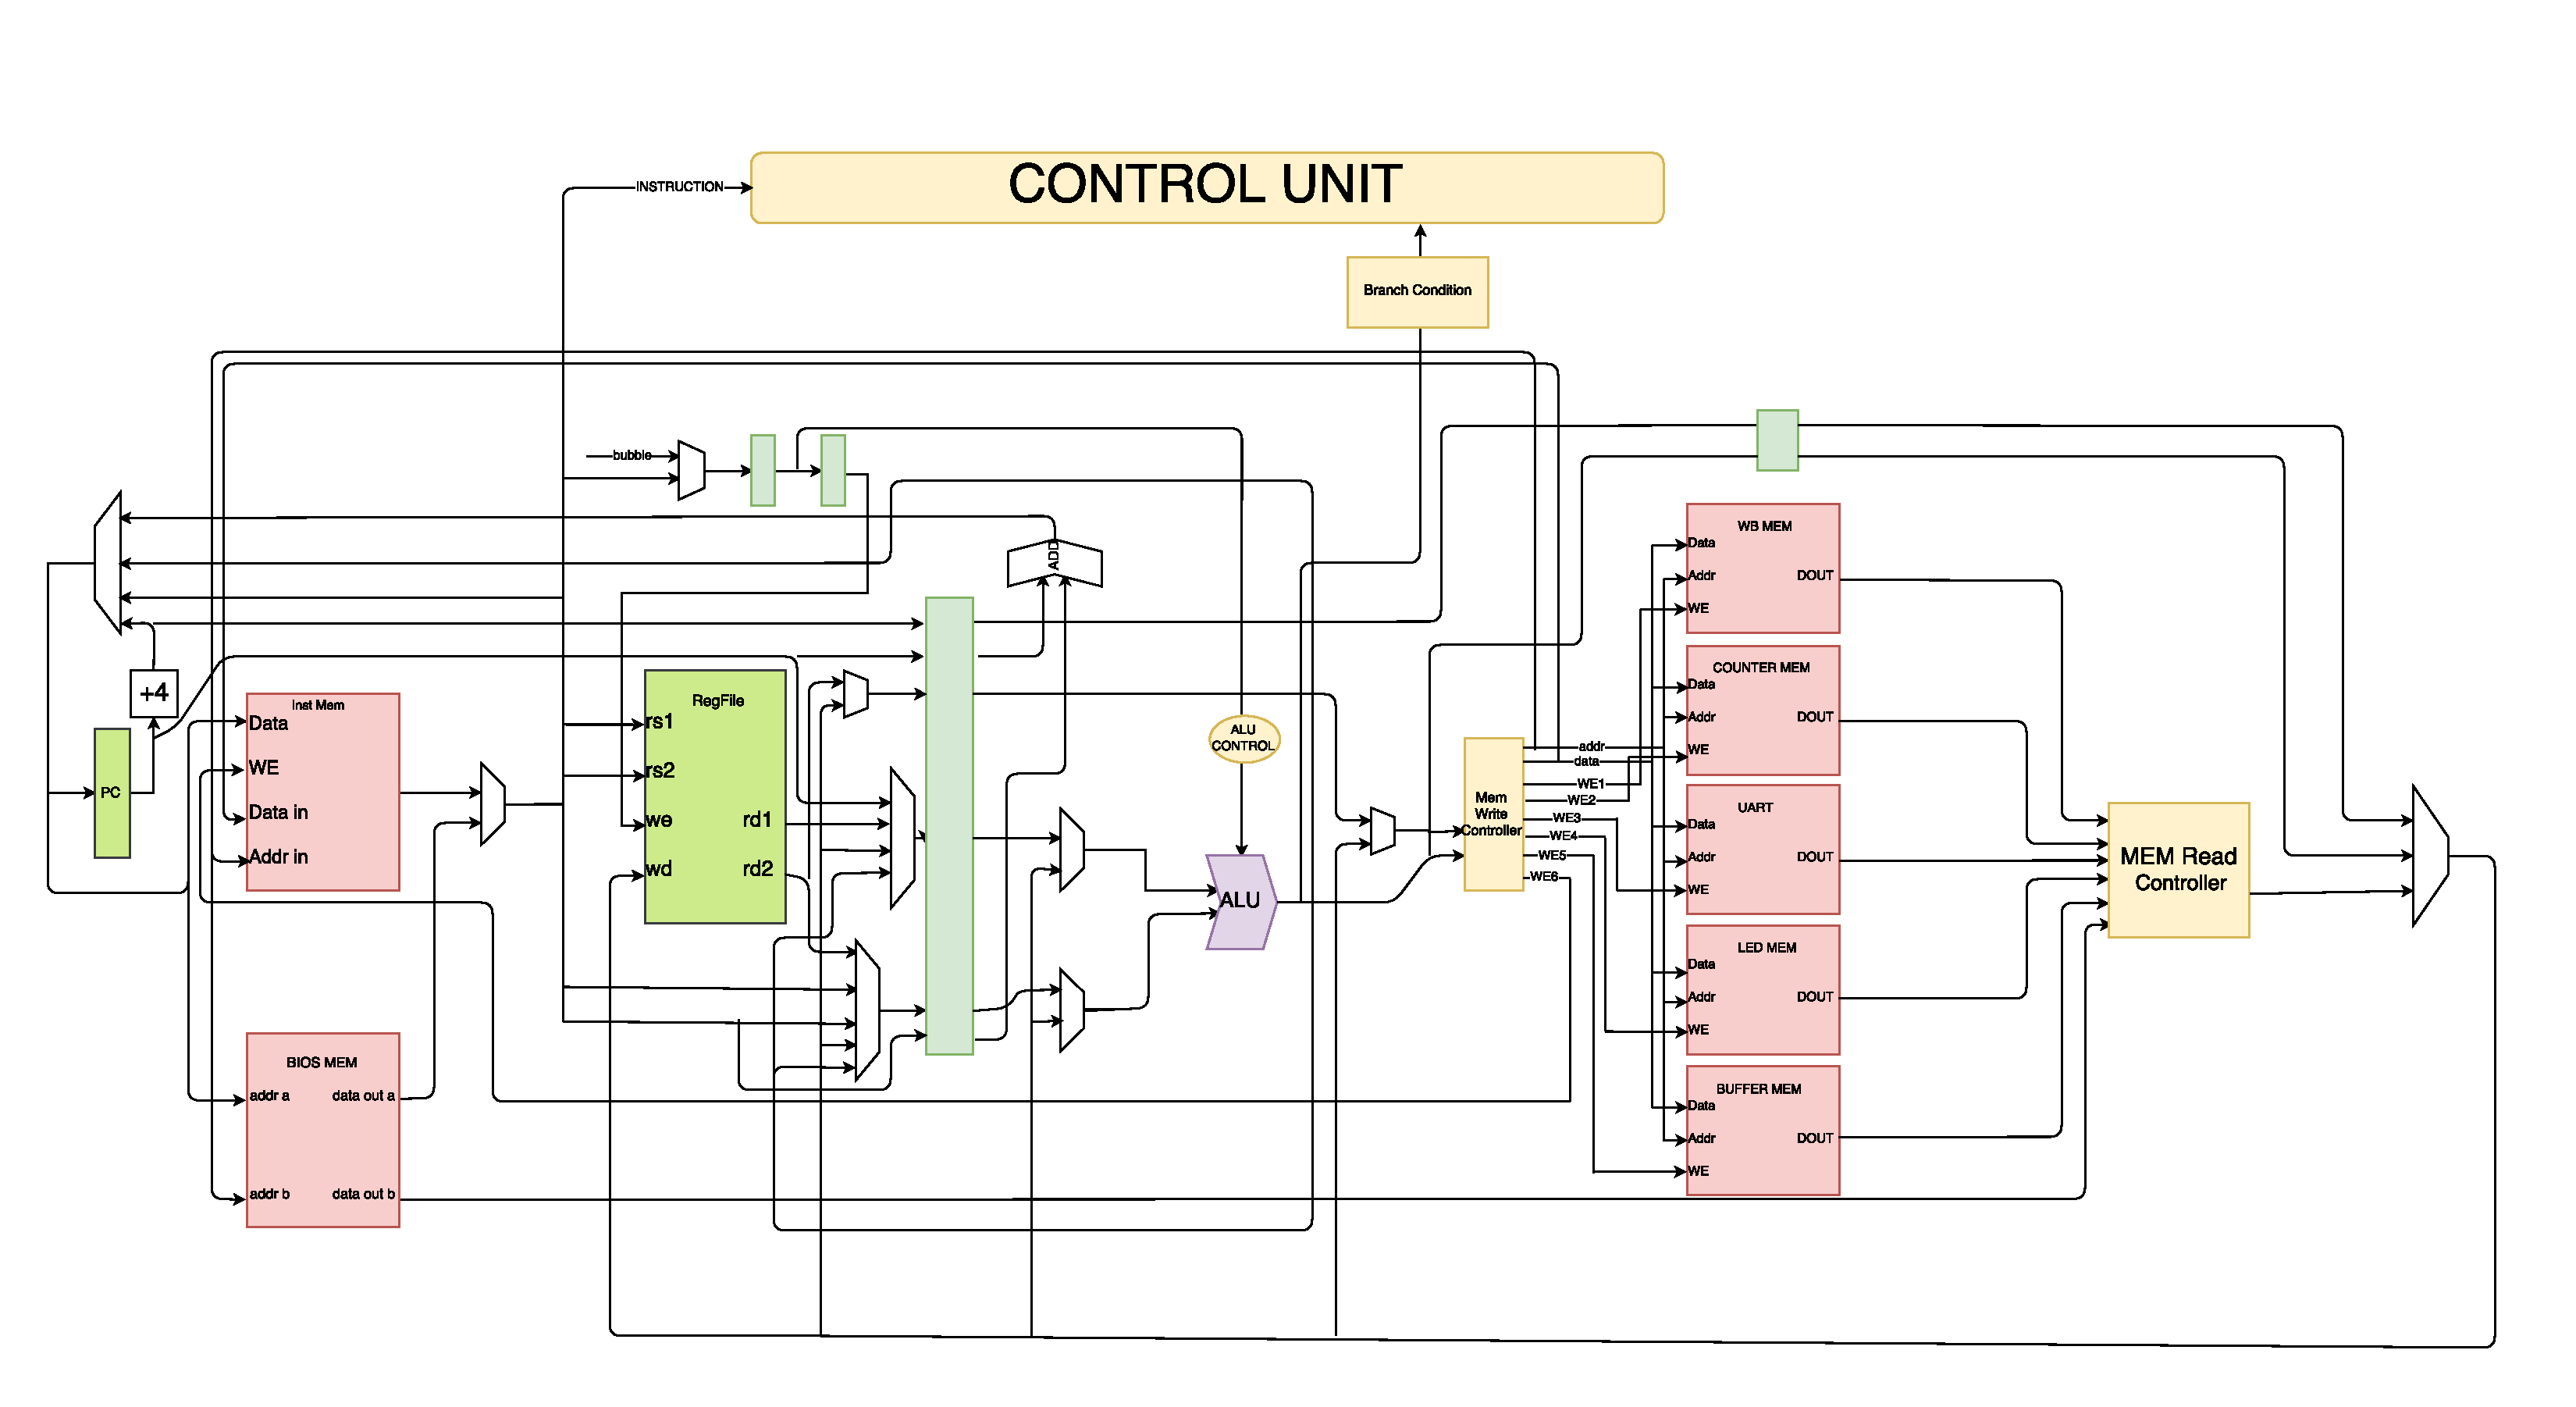
\includegraphics[scale = 0.32, angle=90]{datapath_Diagram.pdf}
\caption{Block diagram of the three stage pipeline}
\label{fig:block-diagram}
\end{figure}


\section{Detailed description of modules}
\subsection{Stage 1: Instruction Fetch and Decode}
In the first stage, the instruction is read out of the instruction memory. The BIOS memory and the instruction memory are in parallel and there is a multiplexer, which is controlled by bit 31 of the program counter, which decides if the instruction from the instruction memory or the BIOS memory should be executed. Because all the memories are synchronous, it is important that the address input should be the address of the next instruction to execute, not the current one. So the address should be pc+4, not just pc. \\\\
After the instruction was read from the instruction memory, it gets decoded. This means that the registers specified by the instructions are read from the register files. These are asynchronous reads, so the data is available at the output shortly after the instruction is set at the input of the register file.

\subsection{Stage 2: Execute}
In the second stage, the instruction gets executed. There are two multiplexers, one for each input of the ALU, which are controlled by the control unit (\ref{sub:control-unit}). These multiplexers forward either the register output or the correct immediate, depending on the instruction, to the input of the ALU. They can also forward the output of the previous operation to the ALU if necessary. The ALU is controlled by the ALU controller, which takes in the instruction and passes an opcode to the ALU, which then executes the correct operation.\\\\
Also in the second stage, the branch address is calculated by a dedicated adder, which adds the pc and the immediate and the branch condition is calculated by the ALU.\\\\
Because the memories are synchronous, the memory write controller is also in the second stage. It takes in the data, which is either the output of the register file or the forwarded output of the previous operation if there is a data hazard, and it creates write enables for the different memories and IO devices depending on the memory map. It also creates a data out signal, which contains the data that should be written to the memory. This is necessary because the memory is byte addressed but the brams can only be accessed one word at a time. So the memory-write-controller takes the data and shifts it to the corresponding byte, depending on the type of store instruction (store byte / halfword / word) and the lowest two address bits.


\subsection{Stage 3: Memory and Writeback}
The output of the ALU gets connected to the address input of the memories and the output of the memory-write-controller to the data input and the write enable. The output of all memories and IO devices then goes into the memory-read-controller, which forwards the data from the correct device depending on the memory map and shifts / sign extends the data depending on the type of the load instruction (signed / unsigned, byte / halfword / word).\\
The writeback multiplexer, which is also controlled by the control unit then chooses which data to write back to the register file depending on the instruction.

\subsection{Control unit}
\label{sub:control-unit}
The control unit is a separate module which computes the control signals for all multiplexers in the ALU. It checks for data and control flow hazards by comparing the instructions in the different stages and sets the multiplexers to forward data if necessary.
\subsubsection{Hazards}
The control unit detects the following data hazards:
\begin{itemize}
\item Instruction depends on the result of the previous instruction. The data gets forwarded from stage three to stage two.
\item Instruction depends on the result of the second to last instruction. This is a hazard because the register file is synchronous write, so the read in the first stage does not return the correct result from the third stage but the value that was stored in the register file. The data gets forwarded from the third to the first stage.
\item Similar to the first two cases, but the second instruction is a store instruction, so not the input of the ALU but the input to the memories needs to be forwarded. The data from the third stage is forwarded to the first or second stage.
\end{itemize}


\subsubsection{Branch prediction}
The control unit also performs a naive form of static branch prediction. We always assume that a branch is not taken. This means that when there is a branch instruction, we always fetch the next instruction and if the branch is taken, which we know after the branch condition gets evaluated in the second stage, we kill the instruction in the first stage. This behavior can be seen in the waveform in fig. \ref{fig:branch-taken}. The \texttt{LW} instruction is fetched in the first stage but once the branch condition is evaluated, the instruction is killed and the instruction at the branch address is fetched next. If the branch is not taken, we just continue execution and no stall or kill is necessary. This can be seen in fig. \ref{fig:branch-not-taken}. The \texttt{LW} instruction after the branch gets fetched in the first stage and then executed as usual, because the branch is not taken.

\begin{figure}[!hbtp]
\centering
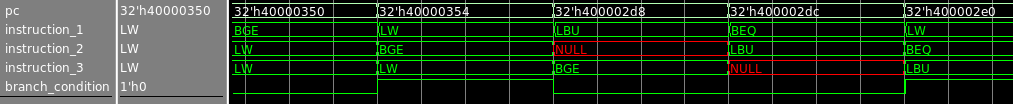
\includegraphics[scale=0.35]{branch.png}
\caption{Waveform of a branch that is taken, one instruction is killed}
\label{fig:branch-taken}
\end{figure}


\begin{figure}[!hbtp]
\centering
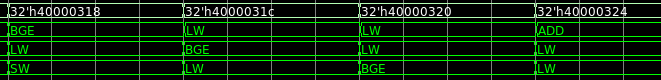
\includegraphics[scale=0.38]{branch-not.png}
\caption{Waveform of a branch that is not taken, no stall / kill necessary}
\label{fig:branch-not-taken}
\end{figure}

\subsection{AC97 Controller}
The AC97 controller is connected to the ALU with two asynchronous FIFOs, one for the sample output and one for the microphone input. These FIFOs can be accessed by the CPU as memory mapped IO. The CPU writes to the sample FIFO and reads from the microphone FIFO, the AC97 controller reads from the sample FIFO and writes to the microphone FIFO. The asynchronous FIFO is, similar to the bram memories, synchronous read, so the read enable gets set when the load instruction is in the second stage, so that the data is available when the instruction is in the writeback stage.\\
The control registers of the AC97 controller are set in a continuous loop. With each frame, one control register gets set to the correct value.

\subsubsection{AC97 Controller output}
The AC97 controller consists of a bit counter, which counts how many bits of the current frame have been sent so far. At the end of a frame, a new sample is read from the asynchronous sample FIFO, which then gets sent out in the next frame. If the FIFO is empty, the previous sample is sent again. The frame gets shifted out over the serial output at the positive edge of the bit clock.

\subsubsection{AC97 Controller microphone input}
The serial input is sampled at the negative edge of the clock input. To enable the microphone input, the corresponding registers have to be set. To do that, they are included in the control loop, which sets one control register every cycle. There is a second bit counter for the input bits, which gets reset every time the sync signal gets set. Once a full frame was received, it is written to the asynchronous microphone FIFO.

\subsection{DVI Controller}
The DVI Controller consists of two counters, one for the vertical and one for the horizontal position. Depending on the values of the counters, the v, h, and de signals are set for the front- and back-porch. There is also a pixel counter, which acts as the address to the framebuffer. It gets incremented whenever the horizontal and vertical counters are in the visible area and it gets reset when a frame is completed.
The framebuffer can be accessed from the CPU as memory mapped IO.


\section{Status and Result}
\subsection{Status}
Our CPU is fully functional. Hazards are handled correctly. However, the microphone input is not working on the board. In the simulation, it seems to be working fine but it does not work on the hardware. To test the microphone input in the simulation, we changed the AC97 codec model to send out data in the microphone slot over the serial data line and verified that the correct data was written into the microphone FIFO with the waveform. This works fine, however it did not work on the board. To find the error, we extended the output of the AC97 controller to include the status registers of the received frame and and used print statements to show the received frame. This showed that we do receive a valid AC97 frame and the valid bits are high for the microphone slots. However, the data in the microphone slot was not changing when we spoke into the microphone.

\subsection{Performance}
For the performance evaluation we removed the I2C controller from our design. This is because the data in the I2C controller changes on the negative edge of the clock, so it only has half a cycle to propagate through the critical path, which leads to a much lower frequency. Therefore, we excluded the I2C controller for the performance evaluation to find the critical path within our CPU and the maximum frequency of it. The I2C controller however still works at the highest possible CPU frequency when running on the board.\\
The maximum frequency of our processor is 60 MHz. With a frequency of 75 MHz there are some timing errors during synthesis but the matrix multiplication benchmark is still working because the critical path is never used in this benchmark. Our CPI is 1.11, the instruction and clock count can be seen in table \ref{tab:performance}.

\begin{table}[!hbtp]
\centering
\begin{tabular}{|c|c|c|}
\hline
& hex & decimal \\
\hline
Instruction count & 3bb32ea & 62,599,914\\
Cycle count & 4279369 & 69,702,505\\
\hline
\end{tabular}
\caption{Cycle and instruction count of mmult benchmark}
\label{tab:performance}
\end{table}

With these numbers, the total execution time of the matrix multiplication program is:
\begin{gather*}
\frac{69702505}{60 MHz} = \underline{\underline{1.1617s}}
\end{gather*}


The critical path is the path from the bios memory, through the forwarding into the ALU, then into the branch condition, to the next pc and back to the bios memory. This path is used when a branch instruction follows a load instruction that reads from the bios memory and there is a hazard: 

\begin{lstlisting}
lw  X1, 0(X2)       # X2 contains address in bios mem
beq X1, X1, branch 
\end{lstlisting}

The critical path can be seen in figure \ref{fig:crit-path}.

\begin{figure}[!hbtp]
\centering
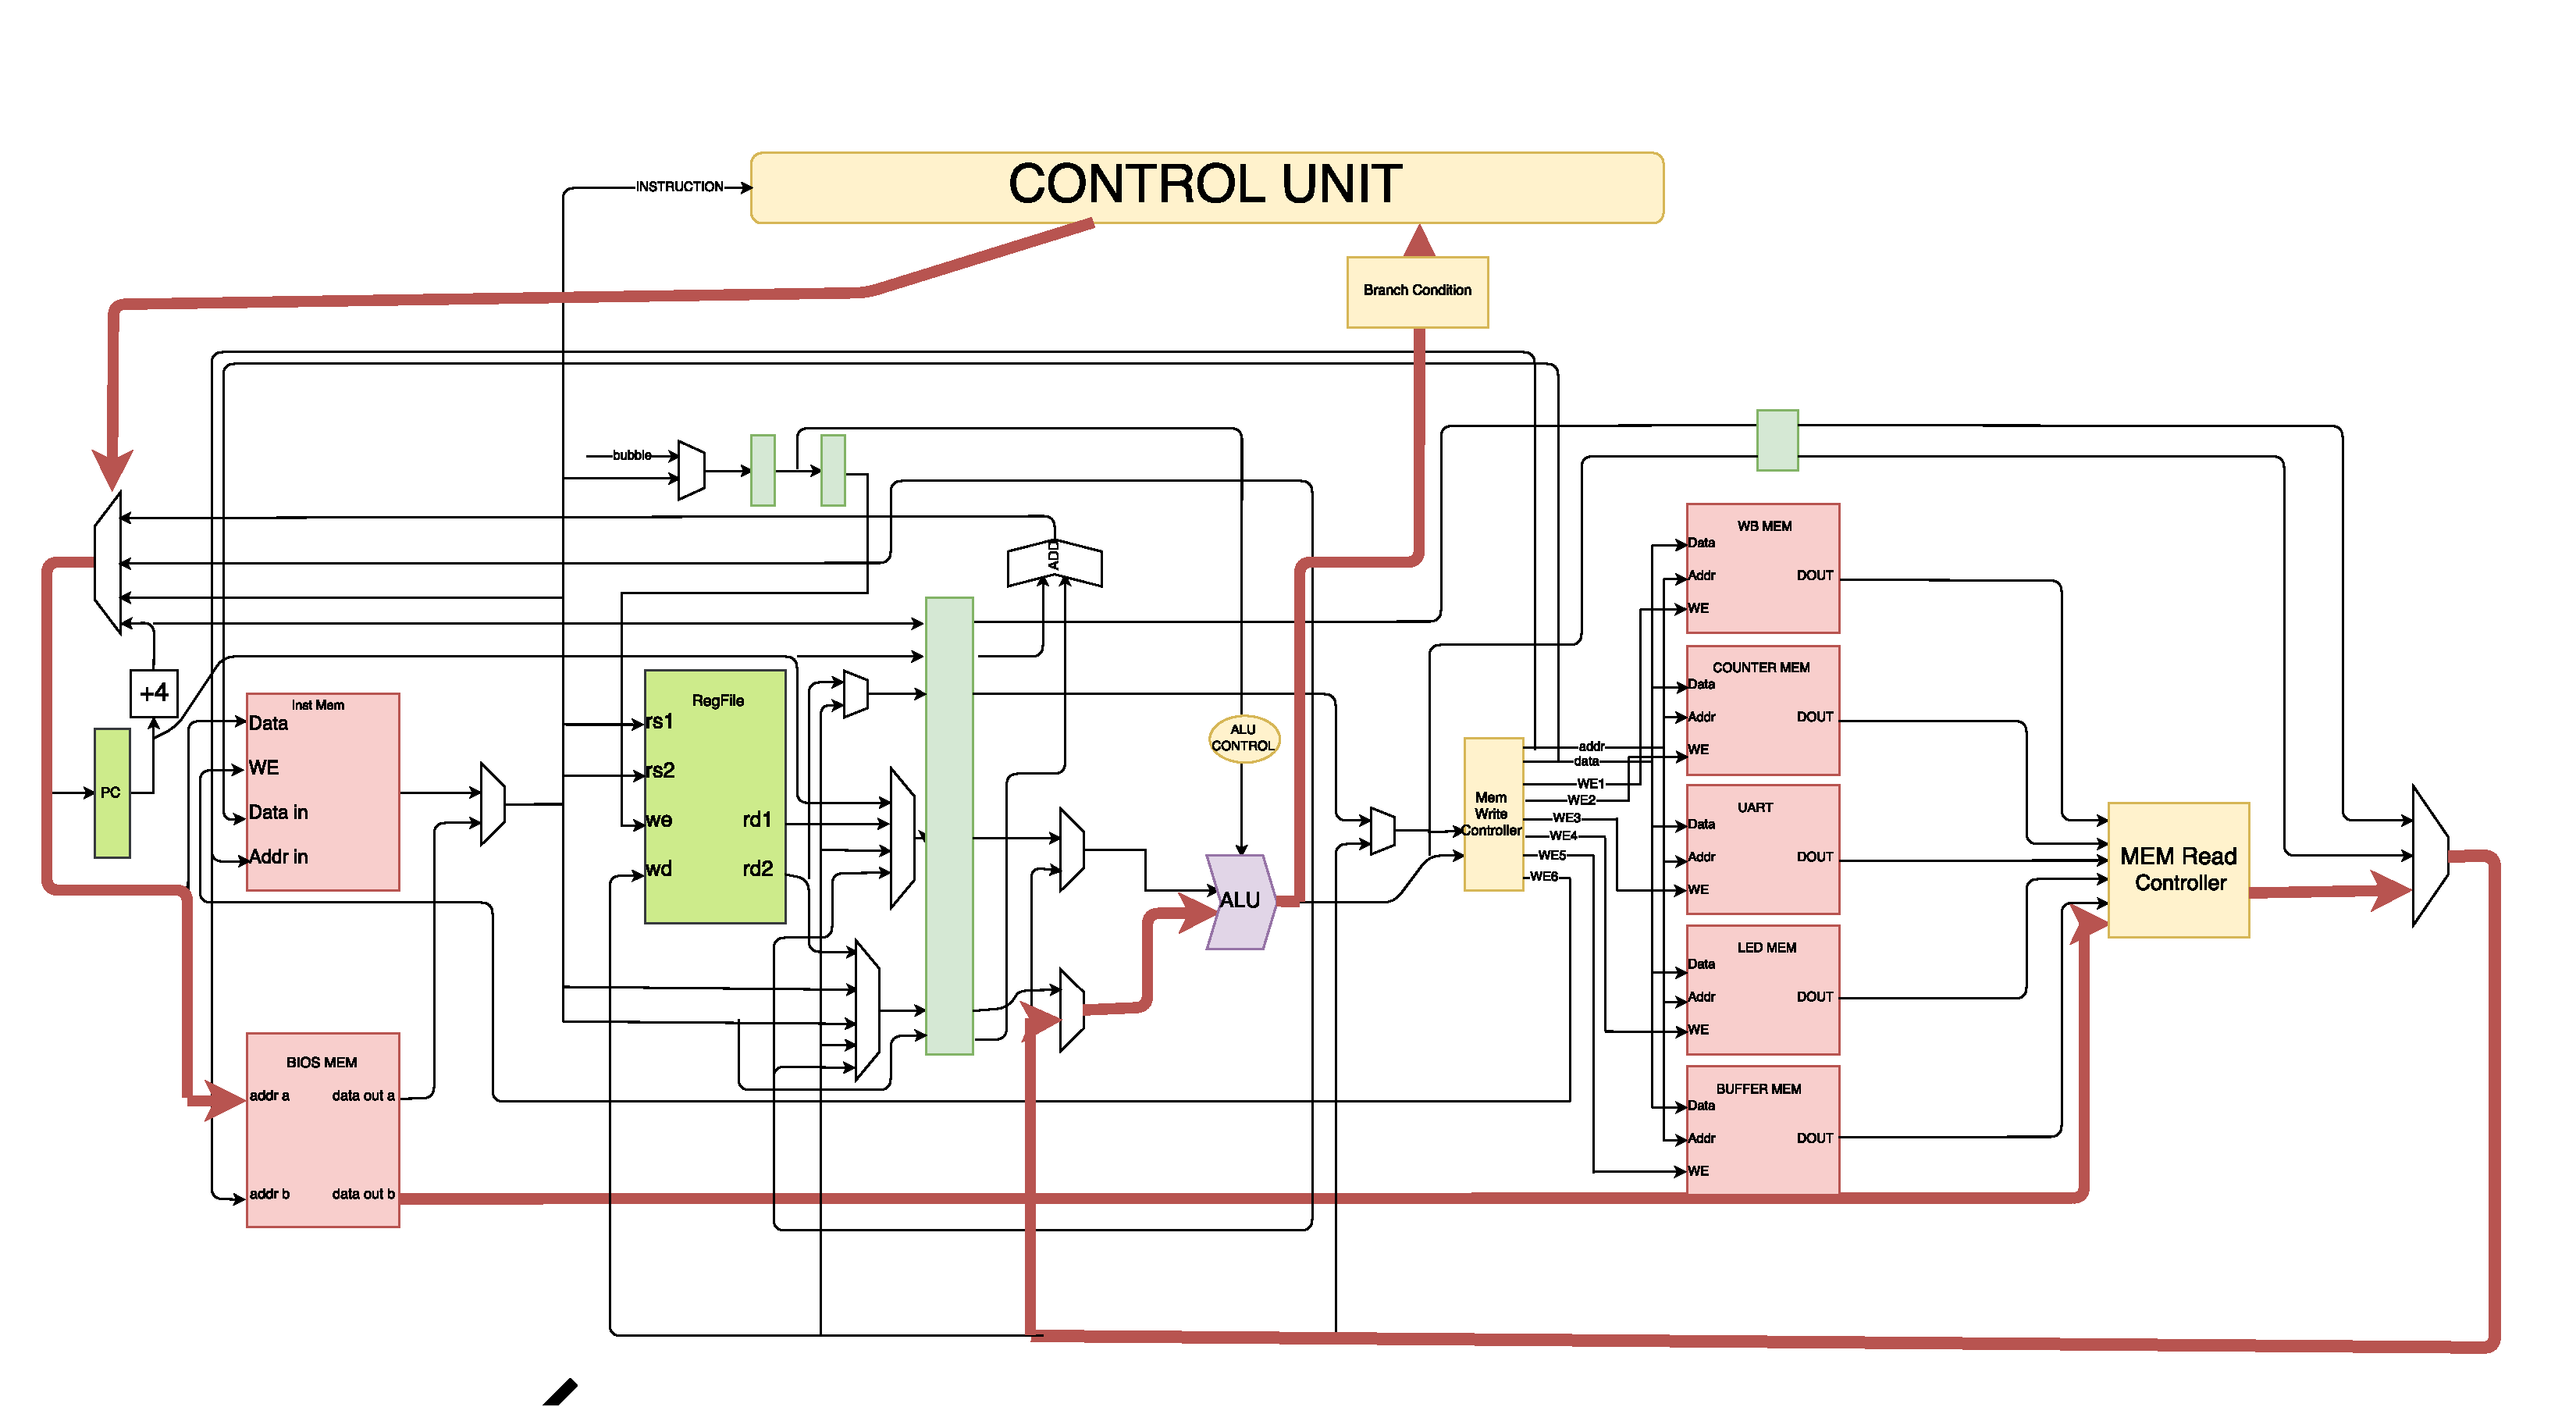
\includegraphics[scale = 0.32, angle = 90]{DiagramCriticalPath.pdf}    
\caption{Block diagram of the critical path}
\label{fig:crit-path}
\end{figure}

\subsection{Resource utilization}
Our entire implementation (including all IO devices) uses the following resources:
\begin{table}[!h]
\centering
\begin{tabular}{|c|c|}
\hline
Slice registers & 2452 \\
\hline 
Slice LUTs & 3469 \\ 
\hline
BlockRAM & 60 \\
\hline
\end{tabular}
\end{table}

\section{Conclusion}
During this project we learned that its very important to separate the design into many small modules. This allows you to have a better overview of how the processors works and it simplifies making changes along the way. \\
We also learned that excessive testing is very hard and time consuming. There are a lot of corner cases, especially when it comes to hazards, so it is hard to make sure that you catch all of them.


\end{document}